\subsection{Methods}
We choose to study the Lunar Lander environment from the gym library. It is slightly more difficult than the cartpole, since it has a larger 
observation space.
The observation space is the following:
$$
O = [x, y, v_x, v_y, \theta, \omega, l_l, l_r]
$$
where $x, y$ are the spatial coordinates, $v_x, v_y$ the velocities, $\theta$ the angle of the lander and $\omega$ its angular velocity. $l_l$
and $l_r$ are boolean variables and are True if the left (right) leg is in contact with the ground. The action space is instead:
$$
A = [null, l_e, c_e, r_e]
$$ 
where $null$ is “do nothing”, $l_e$ is “fire the left engine” and the last two action are respectively fire the central and right engine. The 
fuel is infinite.

The Landing pad starts always at coordinates $(0,0)$. The reward for moving from the top of the screen to landing pad with zero speed is about 
$100-140$ points. If the lander moves away from landing pad it loses reward back. An episode finishes 
if the lander crashes or comes to rest, receiving additional -100 or +100 points. Each leg which makes ground contact is $+10$ reward. 
Firing main engine is $-0.3$ points each frame. The environment is considered solved if the agent reaches $200$ points. 
It is possible to land outside the pad. We show an example of the rendered environment in Figure \ref{fig:Lunar}.

We will use all the tricks explained in Section \ref{sec:cart}.
Since the environment is slightly more difficult than the previous one, we will add another linear layer in the network, using the architecture 
presented in Figure \ref{fig:lun_arc}.
\begin{figure}
    \centering
    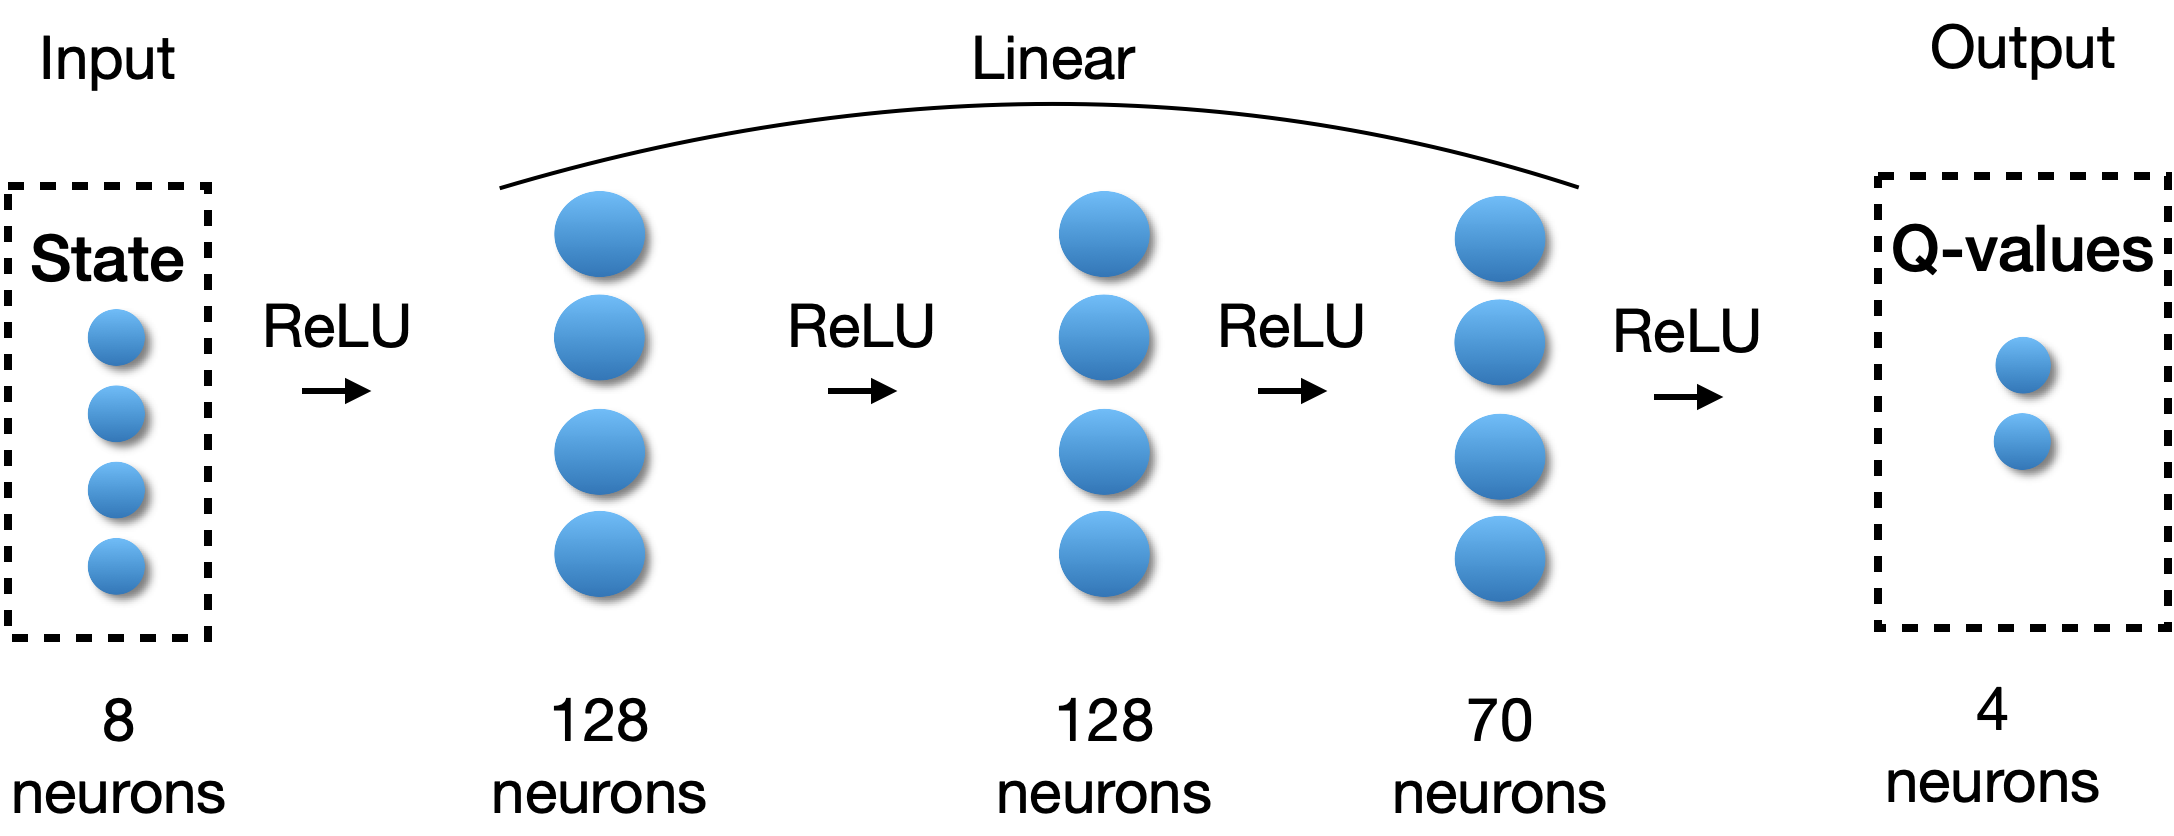
\includegraphics[width=0.7\textwidth]{Images/LunarLandNet.png}
    \caption{Architecture of the network used in the Lunar Lander environment.}
    \label{fig:lun_arc}
\end{figure}


\subsection{Results}
This environment was not trivial to solve. Indeed, to speed up convergence we tried to tweak the reward function. First, we gave some linear malus
if the lander moved away from the center of the screen, i.e.
$$
malus = -\eta |x|
$$
Even though the lander remained in the center of the screen it learned to fly indefinitely. Instead, adding a linear bonus for going downward, i.e.
$$
bonus = -\alpha v_y \theta(-v_y),
$$ 
where $\theta(t)$ is the Heaviside function and $alpha$ is a parameter set to $1.5$, helped in the convergence. In particular, we observe the average score and the exploration path in 
Figure \ref{fig:score_lunar}, and we can observe that it solves the environment at about $800$ steps. We can also observe that the score increases significantly at $600$ iterations after
a plateau, in correspondence to the end of the gaussian addition. This suggests that the increase in the temperature helped to discover a new strategy that was the correct one to solve the 
environment. We can so state that increasing the temperature at later stages of the learning may be useful to improve the final score.
